%%%%%%%%%%%%%%%%%%%%%%%%%%%%%%%%%%%%
% Slide options
%%%%%%%%%%%%%%%%%%%%%%%%%%%%%%%%%%%%

% Option 1: Slides with solutions

\documentclass[slidestop,compress,mathserif]{beamer}
\usepackage{booktabs}
\usepackage{array}
\newcommand{\soln}[1]{\textit{#1}}
\newcommand{\solnGr}[1]{#1}

% Option 2: Handouts without solutions

%\documentclass[11pt,containsverbatim,handout]{beamer}
%\usepackage{booktabs}
%\usepackage{array}
%\usepackage{pgfpages}
%\pgfpagesuselayout{4 on 1}[letterpaper,landscape,border shrink=5mm]
%\newcommand{\soln}[1]{ }
%\newcommand{\solnGr}{ }

%%%%%%%%%%%%%%%%%%%%%%%%%%%%%%%%%%%%
% Style
%%%%%%%%%%%%%%%%%%%%%%%%%%%%%%%%%%%%
%%%%%%%%%%%%%%%%%%%%%%%%%%%%%%%%%%%%%%%%%%%%%%%%%%%%%%%%%%%%%%%%%%%%%%%%
% MA213/214 shared slide style
%
% "Calm & Cool" palette + content-type callout boxes.
% Overhauled (2026) from the original OpenIntro/metropolis style:
%   - all OpenIntro visual branding removed (logo, grid, colors)
%   - a low-key cool palette (see colors below)
%   - tcolorbox callout boxes so students recognize content types
% See common/README.md for the command cheat-sheet.
%%%%%%%%%%%%%%%%%%%%%%%%%%%%%%%%%%%%%%%%%%%%%%%%%%%%%%%%%%%%%%%%%%%%%%%%

\usetheme{metropolis}

%%%%%%%%%%%%%%%%
% Packages
%%%%%%%%%%%%%%%%

\usepackage{geometry}
\usepackage{graphicx}
\usepackage{amssymb}
\usepackage{epstopdf}
\usepackage{amsmath}  	% this permits text in eqnarray among other benefits
\usepackage{url}		% produces hyperlinks
\usepackage{hyperref}	% allows for color usage in tables
\usepackage[english]{babel}
\usepackage[latin1]{inputenc}
\usepackage{colortbl}	% allows for color usage in tables
\usepackage{multirow}	% allows for rows that span multiple rows in tables
\usepackage{color}		% this package has a variety of color options
\usepackage{pgf}
\usepackage{calc}
\usepackage{ulem}
\usepackage{multicol}
\usepackage{textcomp}
\usepackage{txfonts}
\usepackage{listings}
\usepackage{tikz}
\usepackage{array}
\usepackage{wasysym}
\usepackage{fancyvrb}
\usepackage{etoolbox}             % \ifstrempty for optional box subtitles
\usepackage[most]{tcolorbox}      % content-type callout boxes
\tcbuselibrary{listings}          % R-code block (\begin{rblock})
\usepackage{fontawesome5}         % box icons

%%%%%%%%%%%%%%%%
% Remove navigation symbols
%%%%%%%%%%%%%%%%

\setbeamertemplate{navigation symbols}{}

%%%%%%%%%%%%%%%%
% "Calm & Cool" palette
%%%%%%%%%%%%%%%%

% chrome / structure / body
\definecolor{ccSlate}{HTML}{2E3742}   % frametitle bar, structure, section pages (deep neutral slate)
\definecolor{ccInk}{HTML}{2B2B2B}     % body text
\definecolor{ccWash}{HTML}{FCF8F1}    % gentle warm title-slide background wash (complements the cool blues)

% example (blue)
\definecolor{ccBlue}{HTML}{2F6690}
\definecolor{ccBlueBg}{HTML}{EAF1F7}
% interactive activity / discussion (green)
\definecolor{ccGreen}{HTML}{4E8A6B}
\definecolor{ccGreenBg}{HTML}{E9F3EC}
% solution (purple)
\definecolor{ccPurple}{HTML}{6F5499}
\definecolor{ccPurpleBg}{HTML}{EFEAF6}
% worksheet / focused work (terracotta)
\definecolor{ccTerra}{HTML}{C2693E}
\definecolor{ccTerraBg}{HTML}{FAEDE4}
% formula / definition (neutral slate)
\definecolor{ccGray}{HTML}{5C6B7A}
\definecolor{ccGrayBg}{HTML}{EEF1F4}
% caution / common pitfall (brick red)
\definecolor{ccRed}{HTML}{B23A48}
\definecolor{ccRedBg}{HTML}{FAEAEC}
% key idea / takeaway (muted gold)
\definecolor{ccGold}{HTML}{9C7A28}
\definecolor{ccGoldBg}{HTML}{F7F1DF}
% learning goals / lesson outcomes (teal)
\definecolor{ccTeal}{HTML}{2C6E6B}
\definecolor{ccTealBg}{HTML}{E6F0EF}
% learning objectives (indigo)
\definecolor{ccIndigo}{HTML}{45507A}
\definecolor{ccIndigoBg}{HTML}{ECEEF4}
% R code / output (gray)
\definecolor{ccCode}{HTML}{5F5E5A}
\definecolor{ccCodeBg}{HTML}{F4F5F6}

% neutral grays kept from the original style
\definecolor{gray}{rgb}{0.5, 0.5, 0.5}
\definecolor{darkGray}{rgb}{0.3, 0.3, 0.3}
\definecolor{darkerGray}{rgb}{0.2, 0.2, 0.2}

% Backwards-compatible aliases: old OpenIntro color names now point at the
% new palette, so existing \textcolor{oiB}{...}, \hl{...}, etc. keep working.
\colorlet{oiB}{ccBlue}
\colorlet{oiG}{ccGreen}
\colorlet{hlblue}{ccBlue}
\colorlet{rubineRed}{ccRed}
\colorlet{irishGreen}{ccGreen}
\colorlet{lightGreen}{ccGreen}

%%%%%%%%%%%%%%%%
% Restyle metropolis with the Calm & Cool chrome
%%%%%%%%%%%%%%%%

\metroset{block=fill}

\setbeamercolor{normal text}{fg=ccInk, bg=white}
\setbeamercolor{structure}{fg=ccSlate}
\setbeamercolor{alerted text}{fg=ccBlue}
\setbeamercolor{example text}{fg=ccGreen}
\setbeamercolor{frametitle}{bg=ccSlate, fg=white}
\setbeamercolor{progress bar}{fg=ccBlue}
\setbeamercolor{title separator}{fg=ccBlue}
\setbeamercolor{title}{fg=ccSlate}
\setbeamercolor{subtitle}{fg=ccBlue}
\setbeamercolor{author}{fg=ccInk}
\setbeamercolor{institute}{fg=ccGray}
\setbeamercolor{date}{fg=ccGray}
\setbeamercolor{section title}{fg=ccSlate}
\setbeamercolor{standout}{fg=white, bg=ccSlate}

% Section pages sit on the same warm wash as the title slide. We keep
% metropolis's section-title styling and just paint a full-page ccWash
% background behind it (needs >=2 pdflatex passes for the current-page node).
\setbeamertemplate{section page}{%
  \begin{tikzpicture}[remember picture, overlay]
    \fill[ccWash] (current page.south west) rectangle (current page.north east);
  \end{tikzpicture}%
  \centering
  \begin{minipage}{22em}
    \raggedright
    \usebeamercolor[fg]{section title}%
    \usebeamerfont{section title}%
    \insertsectionhead\\[-1ex]
    \usebeamertemplate*{progress bar in section page}%
    \par
  \end{minipage}\par
  \vspace{\baselineskip}
}

%%%%%%%%%%%%%%%%
% Custom inline text commands (recolored to the palette)
%%%%%%%%%%%%%%%%

% degree
\newcommand{\degree}{\ensuremath{^\circ}}

% cite
\newcommand{\ct}[1]{
\vfill
{\tiny #1}}

\newcommand{\NamedNote}[2]{
\rule{2.5cm}{0.25pt} \\ \textit{\footnotesize{\textcolor{rubineRed}{#1:} \textcolor{darkerGray}{#2}}}}

% Note
\newcommand{\Note}[1]{
\rule{2.5cm}{0.25pt} \\ \textit{\footnotesize{\textcolor{rubineRed}{Note:} \textcolor{darkerGray}{#1}}}}

% Remember
\newcommand{\Remember}[1]{\textit{\scriptsize{\textcolor{ccTerra}{Remember:} #1}}}

% expected counts
\newcommand{\ex}[1]{\textit{\textcolor{ccBlue}{#1}}}

% red
\newcommand{\red}[1]{\textit{\textcolor{rubineRed}{#1}}}

% pink
\newcommand{\pink}[1]{\textit{\textcolor{rubineRed!90!white!50}{#1}}}

% green
\newcommand{\green}[1]{\textit{\textcolor{irishGreen}{#1}}}

% orange
\newcommand{\orange}[1]{\textit{\textcolor{ccTerra}{#1}}}

% links: webURL, webLink, appLink
\newcommand{\webURL}[1]{\urlstyle{same}{ \textit{\textcolor{darkGray}{\url{#1}}}}}
\newcommand{\webLink}[2]{\href{#1}{\textcolor{darkGray}{{#2}}}}
\newcommand{\appLink}[2]{\href{#1}{\textcolor{white}{{#2}}}}

% mail
\newcommand{\mail}[1]{\href{mailto:#1}{\textit{\textcolor{darkGray}{#1}}}}

% highlighting: hl, hlGr, mathhl
\newcommand{\hl}[1]{\textit{\textcolor{hlblue}{#1}}}
\newcommand{\hlGr}[1]{\textit{\textcolor{lightGreen}{#1}}}
\newcommand{\mathhl}[1]{\textcolor{hlblue}{\ensuremath{#1}}}

%%%%%%%%%%%%%%%%
% Structural helpers (unchanged from the original)
%%%%%%%%%%%%%%%%

% two col: two columns
\newenvironment{twocol}[4]{
\begin{columns}[c]
\column{#1\textwidth}
#3
\column{#2\textwidth}
#4
\end{columns}
}

% slot (for probability calculations)
\newenvironment{slot}[2]{
\begin{array}{c}
\underline{#1} \\
#2
\end{array}
}

% pr: left and right parentheses
\newcommand{\pr}[1]{
\left( #1 \right)
}

% cancel
\newcommand{\cancel}[1]{%
    \tikz[baseline=(tocancel.base)]{
        \node[inner sep=0pt,outer sep=0pt] (tocancel) {#1};
        \draw[red, line width=0.5mm] (tocancel.south west) -- (tocancel.north east);
    }%
}

% removepagenumbers
\newcommand{\removepagenumbers}{%
  \setbeamertemplate{footline}{}
}

% change margin
\newenvironment{changemargin}[2]{%
\begin{list}{}{%
\setlength{\topsep}{0pt}%
\setlength{\leftmargin}{#1}%
\setlength{\rightmargin}{#2}%
\setlength{\listparindent}{\parindent}%
\setlength{\itemindent}{\parindent}%
\setlength{\parsep}{\parskip}%
}%
\item}{\end{list}}

% footnote
\long\def\symbolfootnote[#1]#2{\begingroup%
\def\thefootnote{\fnsymbol{footnote}}\footnote[#1]{#2}\endgroup}

% commands from the book
\newenvironment{data}[1]{\texttt{#1}}{}
\newenvironment{var}[1]{\texttt{#1}}{}
\newenvironment{resp}[1]{\texttt{#1}}{}

%%%%%%%%%%%%%%%%
% Content-type callout boxes (tcolorbox)
%
% Each type has a colored title strip (icon + label) over a light fill.
% Color = content type; the label + icon reinforce it (so the cue does
% not rely on color alone).
%%%%%%%%%%%%%%%%

\tcbset{
  cccallout/.style 2 args={
    enhanced, breakable=false,
    colback=#2, colframe=#1, colbacktitle=#1, coltitle=white,
    fonttitle=\bfseries\footnotesize,
    boxrule=0.6pt, arc=2.5pt, outer arc=2.5pt,
    left=5pt, right=5pt, top=3pt, bottom=3pt, boxsep=2pt,
    toptitle=2pt, bottomtitle=2pt, lefttitle=5pt,
    before skip=5pt, after skip=5pt,
  },
}

% One-off / collection of examples (blue): \workedexample[subtitle]{body}.
% (Named \workedexample, not \example, because beamer defines \example.)
\newtcolorbox{examplebox}[1][]{cccallout={ccBlue}{ccBlueBg},
  title={\faIcon{lightbulb}~~Example\ifstrempty{#1}{}{ \textmd{---}\ #1}}}
\newcommand{\workedexample}[2][]{\begin{examplebox}[#1]#2\end{examplebox}}

% Running-example header (blue): \examplehead{name} at the top of each frame of a
% multi-slide running example. A one-off or a collection of examples uses the
% \workedexample box above instead.
\newcommand{\examplehead}[1]{%
  \vspace{-0.4em}\par\noindent\tcbox[on line, colback=ccBlue, colframe=ccBlue, coltext=white,
    boxrule=0pt, arc=2pt, left=5pt, right=5pt, top=1pt, bottom=1pt,
    box align=base, nobeforeafter]{\footnotesize\bfseries\faIcon{lightbulb}\,Running example}%
  \ifstrempty{#1}{}{\enspace{\footnotesize\bfseries\textcolor{ccBlue}{#1}}}%
  \par\nobreak\vspace{-0.6em}{\color{ccBlue}\rule{\linewidth}{0.7pt}}\par\nobreak\vspace{-0.8em}}

% Interactive activity (green): \activity[subtitle]{body}
\newtcolorbox{activitybox}[1][]{cccallout={ccGreen}{ccGreenBg},
  title={\faIcon{users}~~Activity\ifstrempty{#1}{}{ #1}}}
\newcommand{\activity}[2][]{\begin{activitybox}[#1]#2\end{activitybox}}

% Discussion question (green): \dq{body}
\newtcolorbox{dqbox}{cccallout={ccGreen}{ccGreenBg}, title={\faIcon{comments}~~Discussion}}
\newcommand{\dq}[1]{\begin{dqbox}#1\end{dqbox}}

% Solution (purple): \solnbox{body}. Gated by the per-deck \soln toggle, so it
% shows in the instructor build and vanishes from the student handout build.
% (Named \solnbox, not \solution, because beamer already defines \solution.)
\newtcolorbox{solutionbox}{cccallout={ccPurple}{ccPurpleBg}, title={\faIcon{key}~~Solution}}
\newcommand{\solnbox}[1]{\soln{\begin{solutionbox}#1\end{solutionbox}}}

% Worksheet / focused work (terracotta): \worksheet[subtitle]{body}
\newtcolorbox{worksheetbox}[1][]{cccallout={ccTerra}{ccTerraBg},
  title={\faIcon{pencil-alt}~~Worksheet\ifstrempty{#1}{}{ #1}}}
\newcommand{\worksheet}[2][]{\begin{worksheetbox}[#1]#2\end{worksheetbox}}

% Formula / definition (neutral slate). Supports both real usages found in the
% decks: \formula{title}{body} and the bare \formula{body} (title defaults to
% "Formula"). The second group is an optional brace argument.
\newtcolorbox{formulabox}[1][Formula]{cccallout={ccGray}{ccGrayBg},
  title={\faIcon{square-root-alt}~~#1}}
\NewDocumentCommand{\formula}{m g}{%
  \IfNoValueTF{#2}%
    {\begin{formulabox}#1\end{formulabox}}%
    {\begin{formulabox}[#1]#2\end{formulabox}}}

% Common pitfall / caution (brick red): \caution[subtitle]{body}
\newtcolorbox{cautionbox}[1][]{cccallout={ccRed}{ccRedBg},
  title={\faIcon{exclamation-triangle}~~Caution\ifstrempty{#1}{}{ #1}}}
\newcommand{\caution}[2][]{\begin{cautionbox}[#1]#2\end{cautionbox}}

% Key idea / takeaway (muted gold): \keyidea[subtitle]{body}
\newtcolorbox{keyideabox}[1][]{cccallout={ccGold}{ccGoldBg},
  title={\faIcon{star}~~Key idea\ifstrempty{#1}{}{ #1}}}
\newcommand{\keyidea}[2][]{\begin{keyideabox}[#1]#2\end{keyideabox}}

% Learning goals / lesson outcomes (teal): \goals{body}. Sits under the short
% LO headings on the objectives slide; body is the "you should be able to" list.
\newtcolorbox{goalsbox}{cccallout={ccTeal}{ccTealBg}, fontupper=\footnotesize,
  top=1pt, bottom=2pt, boxsep=1pt, before skip=3pt,
  title={\faIcon{bullseye}~~By the end of today, you should be able to\ldots}}
\newcommand{\goals}[1]{\begin{goalsbox}#1\end{goalsbox}}

% Learning objectives (indigo): \objectives{body} -- the formal LO headings,
% shown alongside \goals on the objectives slide.
\newtcolorbox{objectivesbox}{cccallout={ccIndigo}{ccIndigoBg}, fontupper=\small,
  top=1pt, bottom=2pt, boxsep=1pt, before skip=3pt,
  title={\faIcon{clipboard-list}~~Learning objectives}}
\newcommand{\objectives}[1]{\begin{objectivesbox}#1\end{objectivesbox}}

% Defaults for a bare \begin{lstlisting}. Without these it inherits the listings
% package defaults: 11pt type, fixed-width columns (which spaces code out as
% "a g e _ f i t"), and no line breaking, so a long line silently runs off the
% right edge of the slide. A deck that passes its own basicstyle still wins.
% Layout only -- syntax coloring is left to the \begin{rblock} environment.
\lstset{
  basicstyle=\ttfamily\footnotesize, columns=fullflexible,
  breaklines=true, breakindent=1.5em, showstringspaces=false,
  numbers=none, frame=none}

% R code / output (gray): \begin{rblock}[subtitle] ... \end{rblock}
% NOTE: a frame containing an rblock must be declared \begin{frame}[fragile].
\lstdefinestyle{ccR}{
  language=R, basicstyle=\ttfamily\footnotesize, columns=fullflexible,
  breaklines=true, showstringspaces=false, numbers=none, frame=none,
  keywordstyle=\color{ccBlue}, commentstyle=\color{ccGreen!75!black},
  stringstyle=\color{ccTerra}}
\newtcblisting{rblock}[1][]{cccallout={ccCode}{ccCodeBg},
  title={\faIcon{terminal}~~R\ifstrempty{#1}{}{ #1}},
  listing only, listing style=ccR}

% --- Legacy boxes (kept so existing decks compile) ---

% app: application exercise -> alias of activity
\newcommand{\app}[1]{\activity{#1}}

% pq: practice question (green, interactive family)
\newtcolorbox{pqbox}{cccallout={ccGreen}{ccGreenBg}, title={\faIcon{list-ol}~~Practice}}
\newcommand{\pq}[1]{\begin{pqbox}#1\end{pqbox}}

% solnMult: solutions for multiple-choice practice questions (uses \soln toggle)
\newcommand{\solnMult}[1]{
\item[] \vspace{-0.59cm}
\only<1>{\item #1}
\soln{\only<2->{\item \orange{#1}}}
}

%%%%%%%%%%%%%%%%
% De-branded title frame + attribution
%%%%%%%%%%%%%%%%

% Eyebrow line on the title slide; a deck may \renewcommand this.
\newcommand{\coursetag}{MA214: Applied Statistics}

% Attribution: all slides released under CC BY-SA, crediting both the
% instructor (later material) and OpenIntro (basis of the earlier material).
\newcommand{\courseattribution}{%
  Slides by Jonathan H.~Huggins, building on materials from OpenIntro's
  \emph{Introduction to Modern Statistics} (Mine \c{C}etinkaya-Rundel et al.).
  Released under the
  \webLink{http://creativecommons.org/licenses/by-sa/3.0/us/}{CC BY-SA license}.
  Some images included under fair use (educational purposes).}

% \maketitleframe: de-branded title slide (no logo, no grid). Uses the deck's
% \title, \subtitle, and \coursetag.
\newcommand{\maketitleframe}{%
  \addtocounter{framenumber}{-1}%
  {\removepagenumbers
  \setbeamercolor{background canvas}{bg=ccWash}%
  \begin{frame}[plain]
    \vspace*{2.6em}
    {\color{ccSlate}\rule{\textwidth}{2.5pt}}\par\vspace{1.5em}
    {\usebeamerfont{date}\scshape\color{ccGray}\coursetag}\par\vspace{0.55em}
    {\usebeamerfont{title}\color{ccSlate}\inserttitle\par}
    \vspace{0.45em}{\color{ccBlue}\rule{3em}{2.5pt}}\par\vspace{0.7em}
    {\usebeamerfont{subtitle}\color{ccBlue}\insertsubtitle\par}
    \vfill
    {\color{ccGray!55}\rule{\textwidth}{0.4pt}}\par\vspace{0.45em}
    {\tiny\color{ccGray}\courseattribution\par}
    \vspace*{0.4em}
  \end{frame}}}

%%%%%%%%%%%%%%%%
% Graphics
%%%%%%%%%%%%%%%%

\DeclareGraphicsRule{.tif}{png}{.png}{`convert #1 `dirname #1`/`basename #1 .tif`.png}

\graphicspath{ {../../common/} {figures/}  }

%%%%%%%%%%%%%%%%%%%%%%%%%%%%%%%%%%%%
% Preamble
%%%%%%%%%%%%%%%%%%%%%%%%%%%%%%%%%%%%

\title[Lecture 18]{Lecture 18: Conjugate models}
\subtitle{Module 4: Bayesian Statistics}
\author{Jonathan H.~Huggins}
\institute{}
\date{}

\begin{document}

%%%%%%%%%%%%%%%%%%%%%%%%%%%%%%%%%%%%
% Title page
%%%%%%%%%%%%%%%%%%%%%%%%%%%%%%%%%%%%

\maketitleframe

%%%%%%%%%%%%%%%%%%%%%%%%%%%%%%%%%%%%
% Agenda
%%%%%%%%%%%%%%%%%%%%%%%%%%%%%%%%%%%%
% !TEX root =  Lecture18.tex


%%%%%%%%%%%%%%%%%%%%%%%%%%%%%%%%%%%%
% Recap/Agenda
%%%%%%%%%%%%%%%%%%%%%%%%%%%%%%%%%%%%
\begin{frame}
\frametitle{Module 4: Bayesian Statistics}
    \begin{itemize}
        \item \hl{Previously:} Lecture 17 opened this module: priors, Bayes' rule, sequential updating.
        \item \hl{This time:} Lecture 17 spread a prior over five candidate values of $p$. Now the grid becomes a \hl{curve}.
          \begin{itemize}
              \item the \hl{Beta} prior, and why Beta $+$ Binomial hands back a Beta;
              \item what makes a prior \hl{conjugate}, and the one pattern all three models share;
              \item two more families: \hl{Normal-Normal} and \hl{Gamma-Poisson};
              \item how much your prior is worth, measured in observations, and where conjugacy runs out.
          \end{itemize}
        \item \hl{Reading:} Bayes Rules!\ Chapters 3 and 5.
        \item \hl{Homework:}
    \end{itemize}
\end{frame}


%%%%%%%%%%%%%%%%%%%%%%%%%%%%%%%%%%%%
% Learning objectives:
%%%%%%%%%%%%%%%%%%%%%%%%%%%%%%%%%%%%
\begin{frame}
    \frametitle{Lecture Objectives}
    \goals{%
    \begin{itemize}
    \item explain what makes a prior \hl{conjugate} to a likelihood, and derive the Beta-Binomial posterior by multiplying shapes, with no integration;
    \item apply all three update rules (\hl{Beta-Binomial}, \hl{Normal-Normal}, \hl{Gamma-Poisson}) and read their parameters as ``prior successes'' or ``prior observations'';
    \item state the \hl{prior sample size} $n_0$ for each family, and use it to compute the weights on prior and data;
    \item explain why the posterior mean is always a \hl{weighted average} of the prior mean and the MLE, and predict which side it falls on;
    \item say what conjugate models buy you, and \hl{where they run out}.
    \end{itemize}}
\end{frame}


%%%%%%%%%%%%%%%%%%%%%%%%%%%%%%%%%%%%
\begin{frame}
    \frametitle{Lecture Objectives}
    \objectives{%
    \begin{itemize}
    \item \textbf{(M4, LO3)} Conjugate Models
    \end{itemize}}
    \vspace{0.3em}
    {\small Building on, and revisiting:}
    \objectives{%
    \begin{itemize}
    \item \textbf{(M4, LO1)} Bayesian Inference: the prior, likelihood and posterior of Lecture 17, now with the parameter on a continuous scale
    \item \textbf{(M4, LO2)} Comparing Bayesian and Frequentist Approaches: the MLE reappears here as one end of a tug-of-war
    \end{itemize}}
\end{frame}


%%%%%%%%%%%%%%%%%%%%%%%%%%%%%%%%%%%%%%%%%%%%%%%%%%%%%%%%%%%%%%%%%%%%%%%%
\section{From a grid to a curve}

%%%%%%%%%%%%%%%%%%%%%%%%%%%%%%%%%%%%%%%%%%%%%%%%%%%%%%%%%%%%%%%%%%%%%%%%
\begin{frame}
\frametitle{From discrete to continuous parameters}

Lecture 17 pinned the response rate $p$ to five candidate values. In reality $p$ can be \textbf{any} value in $[0,1]$.

\pause
\medskip

So the prior stops being a bar chart and becomes a \hl{curve}, and so does the posterior. Probability is now \textbf{area under the curve}, and ``sums to one'' becomes ``total area is one.''

\pause
\medskip

\formula{Posterior $\propto$ likelihood $\times$ prior}{Nothing else changes. At every value of $p$ we still multiply the prior height by the likelihood, then rescale so the total area comes to one: $f(p \mid x) \;\propto\; L(p ; x)\, f(p)$. The rescaling constant is a fixed number: it does not depend on $p$, so it never changes the \emph{shape}.}

\end{frame}

%%%%%%%%%%%%%%%%%%%%%%%%%%%%%%%%%%%%%%%%%%%%%%%%%%%%%%%%%%%%%%%%%%%%%%%%
\section{The Beta-Binomial model}

%%%%%%%%%%%%%%%%%%%%%%%%%%%%%%%%%%%%%%%%%%%%%%%%%%%%%%%%%%%%%%%%%%%%%%%%
\begin{frame}
\frametitle{The Beta distribution}

We need a prior that lives on $[0,1]$, since $p$ is a probability. The \hl{Beta distribution} is a flexible family that does exactly that, governed by two \textbf{shape parameters} $\alpha > 0$ and $\beta > 0$.

\pause
\medskip

If $p \sim \text{Beta}(\alpha, \beta)$, its density is
\[
f(p) \;\propto\; p^{\alpha - 1}(1 - p)^{\beta - 1}.
\]
\pause
There is a normalizing constant out front, but you never need it. What matters is the \textbf{shape}, $p^{\alpha-1}(1-p)^{\beta-1}$.

\end{frame}

%%%%%%%%%%%%%%%%%%%%%%%%%%%%%%%%%%%%%%%%%%%%%%%%%%%%%%%%%%%%%%%%%%%%%%%%
\begin{frame}
\frametitle{Shapes of the Beta distribution}

\begin{center}
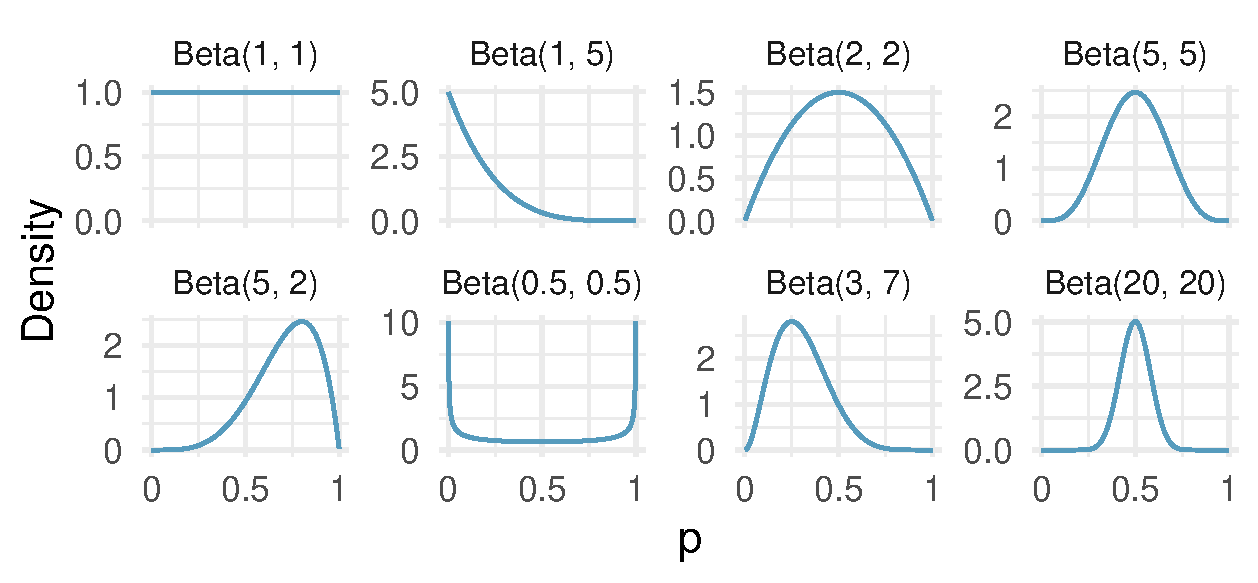
\includegraphics[width=0.94\textwidth]{beta_shapes.pdf}
\end{center}

\vspace{-0.3em}
{\small
\begin{itemize}
\item $\alpha = \beta = 1$: flat, no prior preference at all
\item $\alpha > \beta$ tilts toward large $p$; $\alpha < \beta$ tilts toward small $p$
\item Larger $\alpha + \beta$: more concentrated, a \emph{stronger} prior conviction
\end{itemize}}

\end{frame}

%%%%%%%%%%%%%%%%%%%%%%%%%%%%%%%%%%%%%%%%%%%%%%%%%%%%%%%%%%%%%%%%%%%%%%%%
\begin{frame}
\frametitle{Reading $\alpha$ and $\beta$}

If $p \sim \text{Beta}(\alpha, \beta)$:
\[
E(p) = \frac{\alpha}{\alpha + \beta},
\qquad
\text{Var}(p) = \frac{\alpha\beta}{(\alpha+\beta)^2\,(\alpha+\beta+1)}.
\]
\pause
\keyidea{Read $\alpha$ as ``prior successes'' and $\beta$ as ``prior failures'': the prior behaves like $\alpha + \beta$ observations already seen. That $\alpha+\beta$ is the \hl{strength} of the prior, and sitting in the variance denominator it is what shrinks the spread.}

\pause
\medskip

\textbf{For example:} $\text{Beta}(5,5)$ has mean $0.5$, like having already seen 5 successes and 5 failures. $\text{Beta}(1,1)$ is flat, the weakest prior of all.

\end{frame}

%%%%%%%%%%%%%%%%%%%%%%%%%%%%%%%%%%%%%%%%%%%%%%%%%%%%%%%%%%%%%%%%%%%%%%%%
\begin{frame}
\frametitle{Combining Beta and Binomial}

Combine a Beta prior with the Binomial likelihood from Lecture 17:
\vspace{-0.6em}
\begin{align*}
\text{Prior:} \quad & p \sim \text{Beta}(\alpha, \beta) \\
\text{Data:} \quad & X \mid p \sim \text{Binomial}(n, p)
\end{align*}
\pause
\vspace{-0.8em}

Now just multiply the two shapes together:
\vspace{-0.6em}
\begin{align*}
f(p \mid x) &\propto \underbrace{p^x(1-p)^{n-x}}_{\text{likelihood}} \cdot \underbrace{p^{\alpha-1}(1-p)^{\beta-1}}_{\text{prior}} \\[-0.2em]
&= p^{(\alpha + x) - 1}(1-p)^{(\beta + n - x) - 1}.
\end{align*}
\pause
\vspace{-0.3em}

That is a Beta shape again, with new parameters. No integration, just exponents:
\vspace{-0.6em}
\[
p \mid X = x \;\sim\; \text{Beta}(\alpha + x,\; \beta + n - x)
\]

\end{frame}

%%%%%%%%%%%%%%%%%%%%%%%%%%%%%%%%%%%%%%%%%%%%%%%%%%%%%%%%%%%%%%%%%%%%%%%%
\begin{frame}
\frametitle{The Beta-Binomial update rule}

\[
\text{Beta}(\alpha, \beta) \;\xrightarrow{\;x \text{ successes in } n \text{ trials}\;}\; \text{Beta}(\alpha + x,\; \beta + n - x)
\]
\pause
\medskip

\textbf{Read it as bookkeeping:} start with $\alpha$ prior successes and $\beta$ prior failures, observe $x$ real successes and $n-x$ real failures, and end with $\alpha + x$ and $\beta + n - x$. You just \emph{added them up}.

\pause
\medskip

\caution{Because the update is this cheap, \hl{sequential updating} (Lecture 17) is nearly free here: feed in one batch, then the next, adding to $\alpha$ and $\beta$ each time. Same answer as pooling all the data at once, and as before the order never matters.}

\end{frame}

%%%%%%%%%%%%%%%%%%%%%%%%%%%%%%%%%%%%%%%%%%%%%%%%%%%%%%%%%%%%%%%%%%%%%%%%
\begin{frame}
\frametitle{Example: the drug trial, continuous}

The same Phase 1 trial as Lecture 17, but now $p$ gets a curve, not a grid.

\pause
\medskip

\textbf{Prior:} we expect a low response rate. $\text{Beta}(1, 5)$ encodes that: mean $1/6 \approx 0.167$.

\pause
\medskip

\textbf{Data:} $n = 6$ patients, $x = 2$ respond. The MLE is $\hat p = 2/6 \approx 0.333$, but with only six observations the likelihood is broad: many values of $p$ stay plausible.

\pause
\medskip

\textbf{Posterior:} add them up.
\vspace{-0.3em}
\[
p \mid x = 2 \;\sim\; \text{Beta}(1 + 2,\; 5 + 4) = \text{Beta}(3, 9),
\qquad E(p \mid x) = \tfrac{3}{12} = \hl{0.250}
\]

\end{frame}

%%%%%%%%%%%%%%%%%%%%%%%%%%%%%%%%%%%%%%%%%%%%%%%%%%%%%%%%%%%%%%%%%%%%%%%%
\begin{frame}
\frametitle{Visualizing the update}
\examplehead{Phase 1 drug trial}

\begin{center}
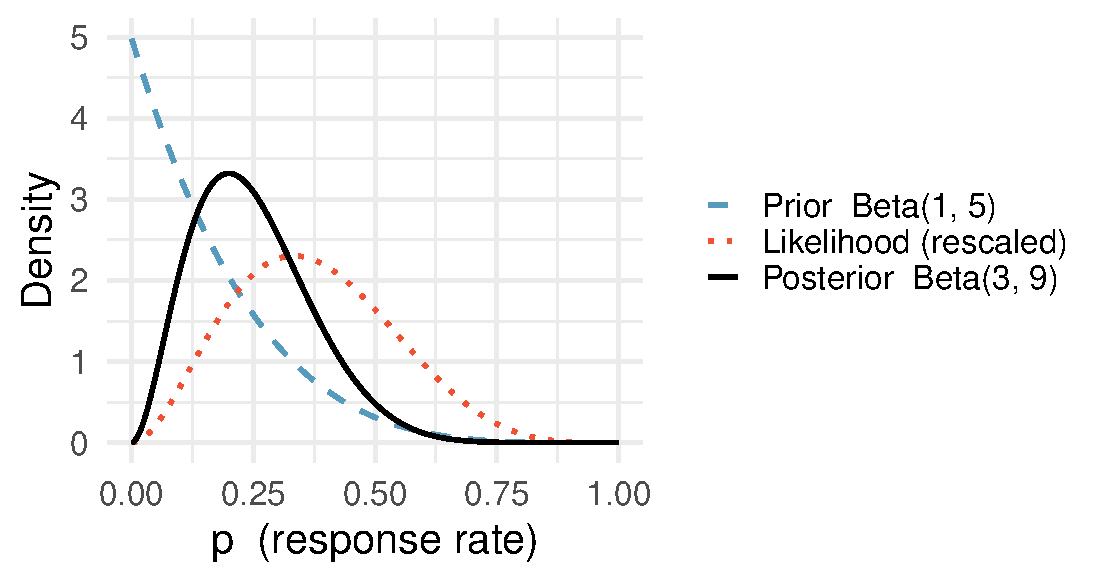
\includegraphics[width=0.84\textwidth]{beta_binomial_update.pdf}
\end{center}

\vspace{-0.3em}
Prior mean $0.167$, MLE $0.333$, posterior mean $0.250$. The posterior lands \emph{between} them.

\end{frame}

%%%%%%%%%%%%%%%%%%%%%%%%%%%%%%%%%%%%%%%%%%%%%%%%%%%%%%%%%%%%%%%%%%%%%%%%
\section{The conjugate pattern}

%%%%%%%%%%%%%%%%%%%%%%%%%%%%%%%%%%%%%%%%%%%%%%%%%%%%%%%%%%%%%%%%%%%%%%%%
\begin{frame}
\frametitle{Two things just happened}
\examplehead{Phase 1 drug trial}

\textbf{One:} the posterior came out in the \emph{same family} as the prior: Beta in, Beta out. When that happens we call the prior \hl{conjugate} to the likelihood.

\pause
\medskip

\textbf{Two:} the posterior mean landed between the prior mean and the MLE, and not arbitrarily:
\vspace{-0.2em}
\[
E(p \mid x) = \frac{\alpha + x}{\alpha + \beta + n}
= \underbrace{\frac{\alpha + \beta}{\alpha + \beta + n}}_{\text{weight on prior}} \cdot \underbrace{\frac{\alpha}{\alpha+\beta}}_{\text{prior mean}}
\;+\; \underbrace{\frac{n}{\alpha + \beta + n}}_{\text{weight on data}} \cdot \underbrace{\frac{x}{n}}_{\text{MLE}}
\]
\pause
\vspace{-0.2em}

Our trial: $\alpha+\beta = 6$ against $n = 6$, so the weights are $0.5$ and $0.5$, and indeed $0.5 \times 0.167 + 0.5 \times 0.333 = 0.250$.

\end{frame}

%%%%%%%%%%%%%%%%%%%%%%%%%%%%%%%%%%%%%%%%%%%%%%%%%%%%%%%%%%%%%%%%%%%%%%%%
\begin{frame}
\frametitle{The weighted-average rule}

\keyidea{In every conjugate model in this lecture, the \hl{posterior mean is a weighted average of the prior mean and the MLE}. The weights are a tug-of-war between a \hl{prior sample size} $n_0$, how many observations the prior is worth, and the real sample size $n$: $\;\text{posterior mean} = \frac{n_0}{n_0+n}\,(\text{prior mean}) + \frac{n}{n_0+n}\,(\text{MLE})$.}

\pause
\medskip

For the Beta-Binomial, $n_0 = \alpha + \beta$. That is the only ingredient that changes when we switch families. The rule itself is unchanged.

\end{frame}

%%%%%%%%%%%%%%%%%%%%%%%%%%%%%%%%%%%%%%%%%%%%%%%%%%%%%%%%%%%%%%%%%%%%%%%%
\begin{frame}
\frametitle{How much is your prior worth?}

Everything follows from comparing $n_0$ against $n$:

\pause
\medskip
\begin{itemize}
\item $n$ \textbf{small} next to $n_0$: the \textbf{prior} dominates, and you brought more conviction than evidence.
\pause
\medskip
\item $n$ \textbf{large} next to $n_0$: the \textbf{data} dominates, and with enough of it the posterior mean is essentially the MLE. \hl{Bayesians and frequentists converge}, the promise from Lecture 17.
\pause
\medskip
\item A \textbf{weak} prior (small $n_0$) is overturned by little data; a \textbf{strong} prior needs a lot of it.
\end{itemize}

\end{frame}

%%%%%%%%%%%%%%%%%%%%%%%%%%%%%%%%%%%%%%%%%%%%%%%%%%%%%%%%%%%%%%%%%%%%%%%%
\begin{frame}
\frametitle{Different people, different priors}
\examplehead{Phase 1 drug trial}

Five oncologists are asked what they believe about the drug's response rate $p$, \emph{before} any trial data:

\pause
\medskip

\begin{itemize}
\item \textbf{Dr.\ Alvarez:} strongly skeptical, expects almost no responders
\item \textbf{Dr.\ Banerjee:} expects a low response rate, like existing drugs
\item \textbf{Dr.\ Chen:} no strong opinion either way
\item \textbf{Dr.\ Diallo:} cautiously optimistic
\item \textbf{Dr.\ Eriksen:} strongly optimistic, expects most patients to respond
\end{itemize}

\pause
\medskip

Encode each as a Beta prior, then run all five through the same update with the same data ($n=6$, $x=2$).

\end{frame}

%%%%%%%%%%%%%%%%%%%%%%%%%%%%%%%%%%%%%%%%%%%%%%%%%%%%%%%%%%%%%%%%%%%%%%%%
\begin{frame}
\frametitle{Five priors, one dataset, five posteriors}
\examplehead{Phase 1 drug trial}

\begin{center}
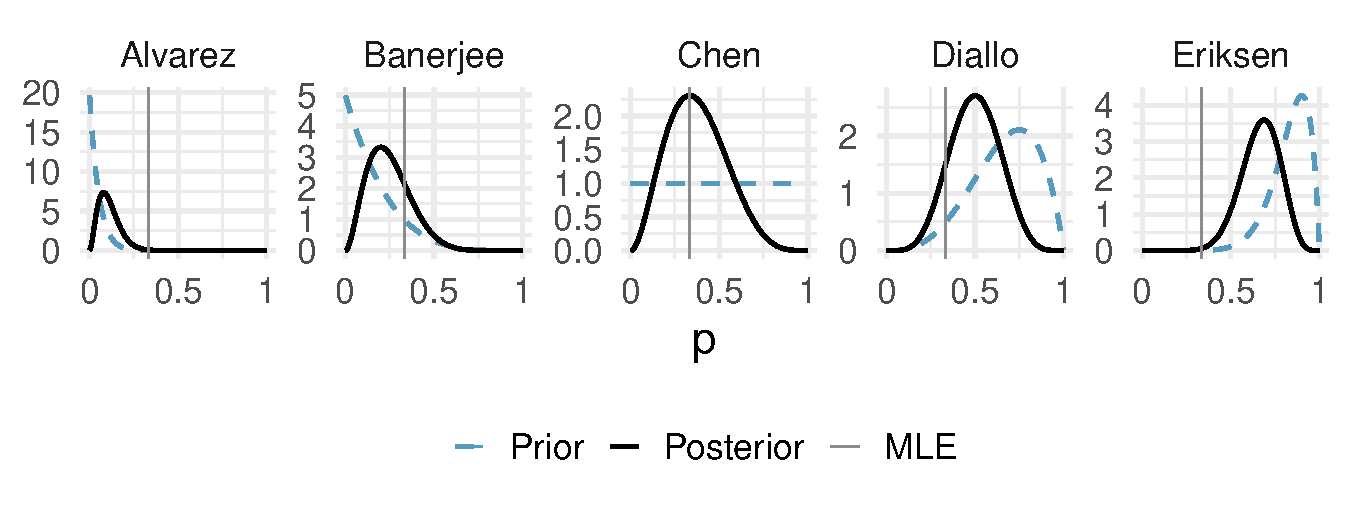
\includegraphics[width=\textwidth]{five_oncologists_grid.pdf}
\end{center}

\end{frame}

%%%%%%%%%%%%%%%%%%%%%%%%%%%%%%%%%%%%%%%%%%%%%%%%%%%%%%%%%%%%%%%%%%%%%%%%
\begin{frame}
\frametitle{Five priors, one dataset, five posteriors}
\examplehead{Phase 1 drug trial}

\begin{center}
{\footnotesize
\renewcommand{\arraystretch}{1.1}
\begin{tabular}{lcccc}
\toprule
Oncologist & Prior & $n_0 = \alpha+\beta$ & Posterior & Post.\ mean \\
\midrule
Dr.\ Alvarez  & $\text{Beta}(1, 20)$ & 21 & $\text{Beta}(3, 24)$ & 0.111 \\
Dr.\ Banerjee & $\text{Beta}(1, 5)$  & 6  & $\text{Beta}(3, 9)$  & 0.250 \\
Dr.\ Chen     & $\text{Beta}(1, 1)$  & 2  & $\text{Beta}(3, 5)$  & 0.375 \\
Dr.\ Diallo   & $\text{Beta}(4, 2)$  & 6  & $\text{Beta}(6, 6)$  & 0.500 \\
Dr.\ Eriksen  & $\text{Beta}(10, 2)$ & 12 & $\text{Beta}(12, 6)$ & 0.667 \\
\bottomrule
\end{tabular}}
\end{center}

\pause
\vspace{-0.2em}
{\small Chen's prior is worth $n_0 = 2$ against $n = 6$ real observations; Alvarez's is worth $21$.}

\pause
\dq{Six patients, five conclusions. Who is doing anything wrong?}

\end{frame}

%%%%%%%%%%%%%%%%%%%%%%%%%%%%%%%%%%%%%%%%%%%%%%%%%%%%%%%%%%%%%%%%%%%%%%%%
\begin{frame}
\frametitle{Six patients, five conclusions}
\examplehead{Phase 1 drug trial}

\textbf{Nobody is doing anything wrong.} Same rule, same data. They differ only in the prior.

\pause
\begin{itemize}
\item Six patients is thin evidence. Their posterior means span $0.11$ to $0.67$; at $n = 200$ that spread collapses to $0.06$.
\pause
\item Each prior is a written-down Beta, so the disagreement is \emph{visible}. A frequentist reports $\hat p = 0.333$ and leaves it unstated.
\end{itemize}

\pause
\keyidea{The prior is where the subjectivity sits, and writing it down is what makes it auditable.}

\end{frame}

%%%%%%%%%%%%%%%%%%%%%%%%%%%%%%%%%%%%%%%%%%%%%%%%%%%%%%%%%%%%%%%%%%%%%%%%
\section{The Normal-Normal model}

%%%%%%%%%%%%%%%%%%%%%%%%%%%%%%%%%%%%%%%%%%%%%%%%%%%%%%%%%%%%%%%%%%%%%%%%
\begin{frame}
\frametitle{Example: birthweight at a rural hospital}

A neonatal researcher wants the mean birthweight $\mu$ (grams) at a rural hospital serving a high-risk population.

\pause
\medskip
\begin{itemize}
\item \hl{National data:} mean $\approx 3300$ g, SD $\sigma = 500$ g \quad (we treat $\sigma$ as known)
\pause
\item \hl{Prior:} this hospital is probably near the national average, so $\mu \sim N(3300, 200^2)$. A prior SD of $200$ g ($\approx 0.45$ lbs) is moderately informative
\pause
\item \hl{Data:} $n = 12$ births here, sample mean $\bar{x} = 2980$ g
\end{itemize}

\pause
\medskip
\dq{The parameter is now a weight in grams, not a probability. Does anything actually change?}

\end{frame}

%%%%%%%%%%%%%%%%%%%%%%%%%%%%%%%%%%%%%%%%%%%%%%%%%%%%%%%%%%%%%%%%%%%%%%%%
\begin{frame}
\frametitle{The Normal likelihood}

With $X_1,\ldots,X_n \mid \mu \stackrel{\text{iid}}{\sim} N(\mu, \sigma^2)$ and $\sigma^2$ known, multiplying the $n$ densities together and keeping only what depends on $\mu$ leaves
\[
L(\mu\,; \mathbf{x}) \;\propto\; \exp\!\left(-\frac{1}{2\sigma^2}\sum_{i=1}^n(x_i - \mu)^2\right).
\]
\pause
The identity $\sum_i (x_i - \mu)^2 = n(\mu - \bar{x})^2 + \sum_i (x_i - \bar{x})^2$ has a second piece free of $\mu$, so this collapses to
\[
L(\mu\,; \bar{x}) \;\propto\; \exp\!\left(-\frac{n}{2\sigma^2}(\mu - \bar{x})^2\right).
\]
\pause
That is a Normal shape in $\mu$, centered at $\bar{x}$. So \hl{the whole sample enters only through $\bar{x}$}.

\end{frame}

%%%%%%%%%%%%%%%%%%%%%%%%%%%%%%%%%%%%%%%%%%%%%%%%%%%%%%%%%%%%%%%%%%%%%%%%
\begin{frame}
\frametitle{The MLE and the shape of the likelihood}
\examplehead{Birthweight}

\begin{center}
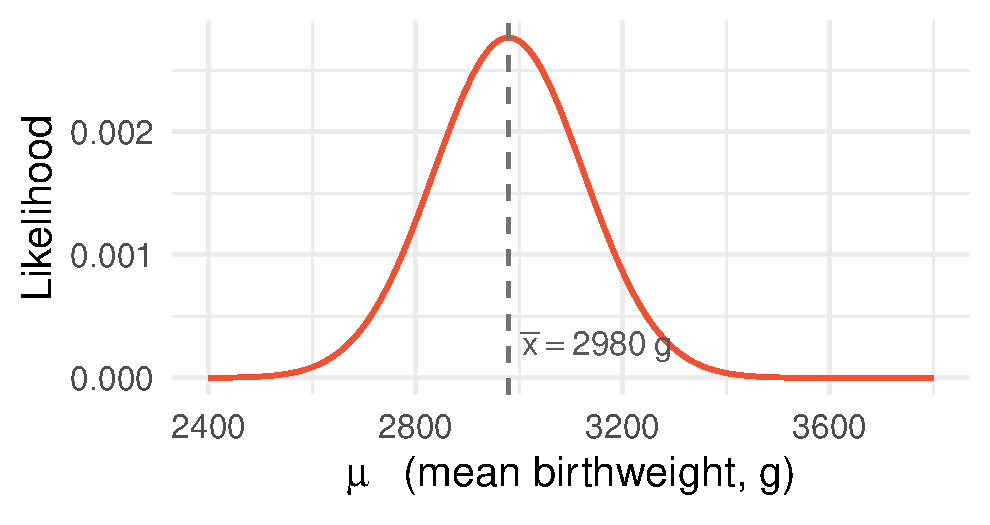
\includegraphics[width=0.74\textwidth]{normal_likelihood_mle.pdf}
\end{center}

\vspace{-0.3em}
{\small The likelihood is largest where $(\mu - \bar x)^2$ is smallest, so $\hat\mu_{\text{MLE}} = \bar{x}$: a squared distance is smallest when it is zero, no calculus needed. Its width is $\sigma/\sqrt{n}$, so more data or a smaller $\sigma$ makes it narrower.}

\end{frame}

%%%%%%%%%%%%%%%%%%%%%%%%%%%%%%%%%%%%%%%%%%%%%%%%%%%%%%%%%%%%%%%%%%%%%%%%
\begin{frame}
\frametitle{The Normal-Normal update}

Put a Normal prior on the parameter: $\mu \sim N(\mu_0, \sigma_0^2)$, with $\mu_0$ the prior mean and $\sigma_0$ how unsure we are. Multiply the two Normal shapes and, as with Beta, a Normal comes out.

\pause
\medskip

\formula{Precisions add}{The \hl{precision} of a distribution is $1/\text{variance}$: high precision means low uncertainty. The prior has precision $1/\sigma_0^2$ and the data has precision $n/\sigma^2$. Writing $\sigma_n$ for the posterior SD, the posterior precision is their sum: $\;\frac{1}{\sigma_n^2} = \frac{1}{\sigma_0^2} + \frac{n}{\sigma^2}$.}

\pause
\medskip

So evidence \emph{accumulates}: every observation adds precision and the posterior can only get narrower.

\end{frame}

%%%%%%%%%%%%%%%%%%%%%%%%%%%%%%%%%%%%%%%%%%%%%%%%%%%%%%%%%%%%%%%%%%%%%%%%
\begin{frame}
\frametitle{The same pattern, in grams}

Define the \hl{prior sample size} $n_0 = \sigma^2/\sigma_0^2$: the number of real births that would carry the same precision as the prior. Then the posterior mean is
\[
\mu_n = \frac{n_0}{n_0 + n}\,\mu_0 + \frac{n}{n_0 + n}\,\bar{x},
\qquad
\sigma_n = \frac{\sigma}{\sqrt{n_0 + n}}.
\]
\pause
\keyidea{This is the \emph{same} weighted average as the Beta-Binomial. Only the recipe for $n_0$ changed: there $n_0 = \alpha + \beta$, here $n_0 = \sigma^2/\sigma_0^2$. The posterior behaves like $n_0 + n$ observations: $n_0$ imagined, $n$ real.}

\end{frame}

%%%%%%%%%%%%%%%%%%%%%%%%%%%%%%%%%%%%%%%%%%%%%%%%%%%%%%%%%%%%%%%%%%%%%%%%
\begin{frame}
\frametitle{Birthweight: prior observations and weights}
\examplehead{Birthweight}

\textbf{Setup:} prior $N(3300, 200^2)$; data $n = 12$, $\bar{x} = 2980$ g, $\sigma = 500$ g.

\pause\smallskip

\textbf{Step 1. How much is the prior worth?}
\vspace{-0.2em}
\[
n_0 = \frac{\sigma^2}{\sigma_0^2} = \frac{500^2}{200^2} = \frac{250{,}000}{40{,}000} = \hl{6.25}
\]
\vspace{-0.4em}

The prior is worth about \hl{6 previously observed births}, against 12 real ones.

\pause\smallskip

\textbf{Step 2. Effective sample size and posterior SD.}
\vspace{-0.2em}
\[
n_0 + n = 6.25 + 12 = 18.25,
\qquad
\sigma_n = \frac{500}{\sqrt{18.25}} \approx \hl{117}\text{ g}
\]

\end{frame}

%%%%%%%%%%%%%%%%%%%%%%%%%%%%%%%%%%%%%%%%%%%%%%%%%%%%%%%%%%%%%%%%%%%%%%%%
\begin{frame}
\frametitle{Birthweight: the posterior}
\examplehead{Birthweight}

\textbf{Step 3. The weighted average.}
\vspace{-0.2em}
\[
\mu_n
  = \underbrace{\tfrac{6.25}{18.25}}_{0.34} \times 3300
  + \underbrace{\tfrac{12}{18.25}}_{0.66} \times 2980
  \approx \hl{3090}\text{ g}
\]
\pause
The 12 births get two thirds of the weight, so the posterior sits nearer the data, though the prior still pulls it $110$ g above $\bar x$.

\pause
\medskip

Since the posterior is Normal, we can read an interval straight off it: $3090 \pm 1.96 \times 117 = (2860,\ 3319)$ g. That is a \hl{credible interval}: an interval $\mu$ falls in with probability $0.95$, given this data. \hl{Lecture 20} makes that precise.

\end{frame}

%%%%%%%%%%%%%%%%%%%%%%%%%%%%%%%%%%%%%%%%%%%%%%%%%%%%%%%%%%%%%%%%%%%%%%%%
\begin{frame}
\frametitle{Visualizing the Normal-Normal update}
\examplehead{Birthweight}

\begin{center}
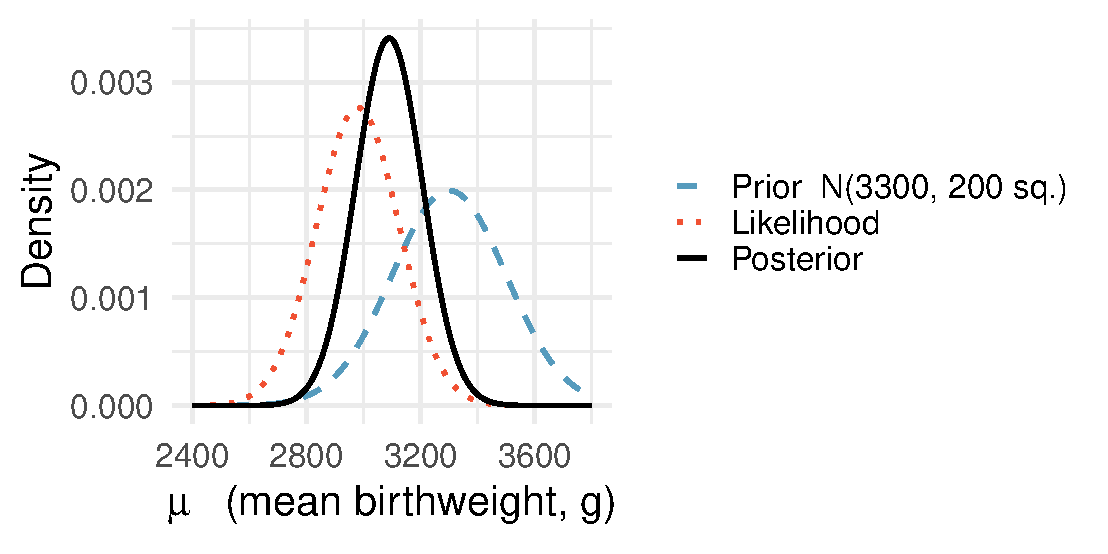
\includegraphics[width=0.86\textwidth]{normal_normal_update.pdf}
\end{center}

\vspace{-0.3em}
Same picture as the drug trial, different units. The posterior is narrower than \emph{both} inputs, because precisions add.

\end{frame}

%%%%%%%%%%%%%%%%%%%%%%%%%%%%%%%%%%%%%%%%%%%%%%%%%%%%%%%%%%%%%%%%%%%%%%%%
\section{The Gamma-Poisson model}

%%%%%%%%%%%%%%%%%%%%%%%%%%%%%%%%%%%%%%%%%%%%%%%%%%%%%%%%%%%%%%%%%%%%%%%%
\begin{frame}
\frametitle{Example: whale sightings off Cape Cod}

A marine biologist is estimating $\lambda$, the rate of whale sightings per day off Cape Cod during spring migration.

\pause
\medskip
\begin{itemize}
\item \hl{Historical records:} about 3 sightings per day
\pause
\item \hl{Data:} over $n = 7$ days they record $5, 2, 4, 6, 3, 7, 4$, so $\sum x_i = 31$ and $\bar{x} = 4.43$/day
\end{itemize}

\pause
\medskip
\dq{Has the sighting rate risen above the historical 3 per day, or is 7 days just noisy?}

\pause
\medskip
A third parameter type: not a probability, not a mean weight, but a \textbf{rate}, any positive number.

\end{frame}

%%%%%%%%%%%%%%%%%%%%%%%%%%%%%%%%%%%%%%%%%%%%%%%%%%%%%%%%%%%%%%%%%%%%%%%%
\begin{frame}
\frametitle{The Poisson distribution}

The \hl{Poisson} models counts with no fixed upper bound: earthquakes per year, goals per match, patients arriving per hour, whales per day.
\[
X \mid \lambda \sim \text{Poisson}(\lambda), \qquad P(X = x \mid \lambda) = \frac{\lambda^x e^{-\lambda}}{x!}, \quad x = 0, 1, 2, \ldots
\]
\pause
\begin{itemize}
\item $\lambda > 0$ is the average event rate, the parameter we want
\pause
\item $E(X) = \lambda$ and $\text{Var}(X) = \lambda$: \hl{mean equals variance}, so busier rates are also more variable
\end{itemize}

\end{frame}

%%%%%%%%%%%%%%%%%%%%%%%%%%%%%%%%%%%%%%%%%%%%%%%%%%%%%%%%%%%%%%%%%%%%%%%%
\begin{frame}
\frametitle{Shapes of the Poisson distribution}

\begin{center}
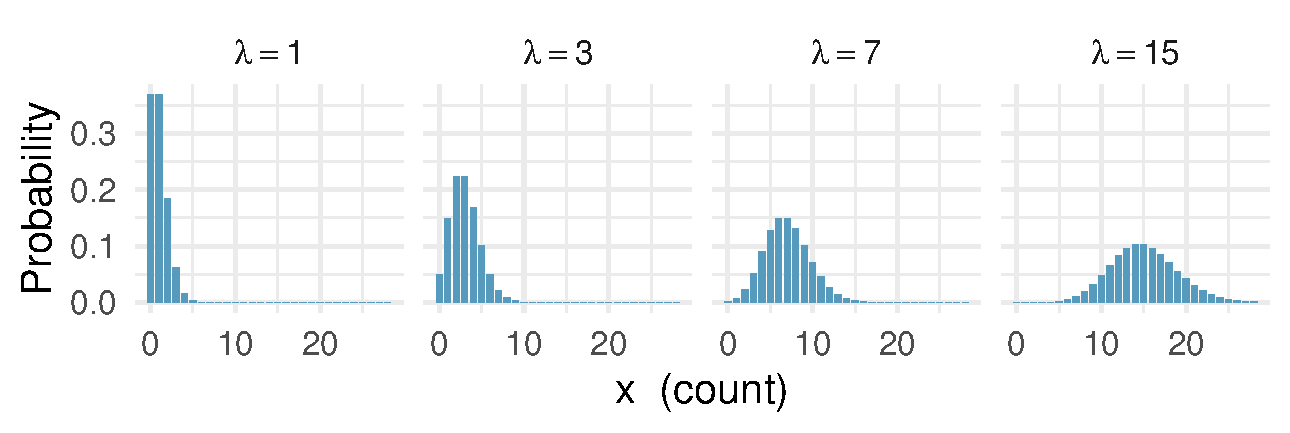
\includegraphics[width=\textwidth]{poisson_pmfs.pdf}
\end{center}

\vspace{-0.2em}
{\small As $\lambda$ grows the distribution shifts right, spreads out, and starts to look symmetric. Note these are bars, not a curve: the \emph{data} is still discrete counts. It is the \emph{parameter} $\lambda$ that gets a continuous prior.}

\end{frame}

%%%%%%%%%%%%%%%%%%%%%%%%%%%%%%%%%%%%%%%%%%%%%%%%%%%%%%%%%%%%%%%%%%%%%%%%
\begin{frame}
\frametitle{The Poisson likelihood}

Multiply the $n$ probabilities together and keep only what depends on $\lambda$:
\[
L(\lambda\,; \mathbf{x}) = \prod_{i=1}^n \frac{\lambda^{x_i} e^{-\lambda}}{x_i!} \;\propto\; \lambda^{\sum x_i}\, e^{-n\lambda}
\]
\pause
So, as with the Normal, the sample enters only through a summary: here the \textbf{total count} $\sum x_i$.

\pause
\medskip

The MLE is the sample mean, $\hat\lambda_{\text{MLE}} = \bar{x}$. For the whales, $\hat\lambda = 31/7 \approx \hl{4.43}$ sightings/day.

\end{frame}

%%%%%%%%%%%%%%%%%%%%%%%%%%%%%%%%%%%%%%%%%%%%%%%%%%%%%%%%%%%%%%%%%%%%%%%%
\begin{frame}
\frametitle{The Gamma distribution}

We need a prior for a rate, so it must live on the positive numbers. The \hl{Gamma distribution} does:
\[
\lambda \sim \text{Gamma}(\alpha, \beta), \qquad f(\lambda) \;\propto\; \lambda^{\alpha - 1} e^{-\beta\lambda}
\]
\pause
\begin{itemize}
\item \textbf{Mean:} $E(\lambda) = \alpha/\beta$; \quad \textbf{Variance:} $\text{Var}(\lambda) = \alpha/\beta^2$
\pause
\item \textbf{Interpretation:} $\alpha$ is a ``prior total count'' and $\beta$ a ``prior number of observations'', so $\beta$ is this family's \hl{prior sample size $n_0$}
\end{itemize}

\pause
\medskip

\dq{Look at that density. Where have you already seen a shape like $\lambda^{\text{something}} e^{-\text{something} \times \lambda}$?}

\end{frame}

%%%%%%%%%%%%%%%%%%%%%%%%%%%%%%%%%%%%%%%%%%%%%%%%%%%%%%%%%%%%%%%%%%%%%%%%
\begin{frame}
\frametitle{Shapes of the Gamma distribution}
\examplehead{Whale sightings}

\begin{center}
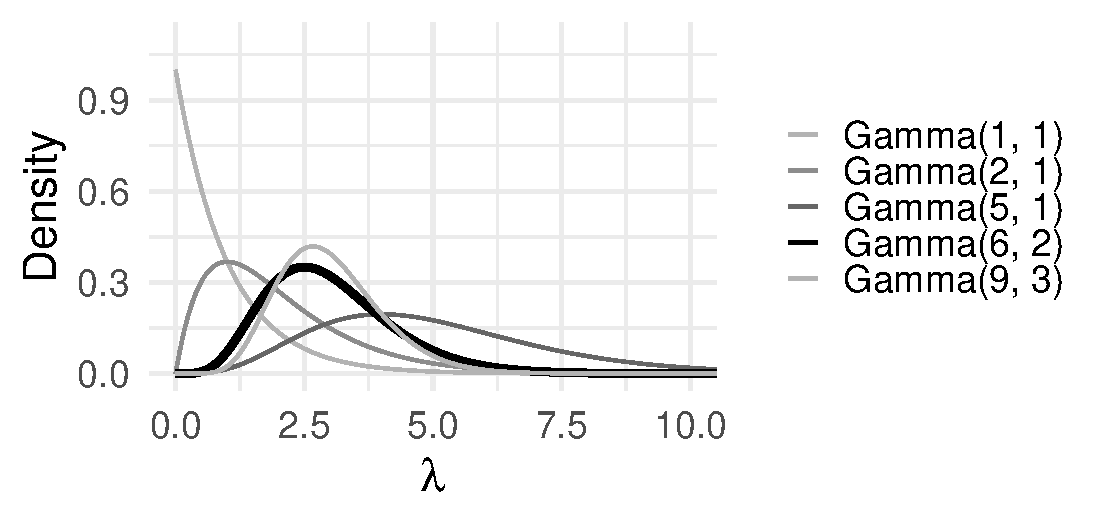
\includegraphics[width=0.86\textwidth]{gamma_shapes.pdf}
\end{center}

\vspace{-0.3em}
The two parameters move the center and the spread independently. $\text{Gamma}(6,2)$ has mean $3$, the historical whale rate, so it is the natural prior here.

\end{frame}

%%%%%%%%%%%%%%%%%%%%%%%%%%%%%%%%%%%%%%%%%%%%%%%%%%%%%%%%%%%%%%%%%%%%%%%%
\begin{frame}
\frametitle{The Gamma-Poisson update}

Multiply the Gamma prior shape by the Poisson likelihood shape:
\[
\underbrace{\lambda^{\alpha-1}e^{-\beta\lambda}}_{\text{prior}} \cdot \underbrace{\lambda^{\sum x_i}e^{-n\lambda}}_{\text{likelihood}}
= \lambda^{(\alpha + \sum x_i) - 1}\, e^{-(\beta + n)\lambda}
\]
\pause
Gamma in, Gamma out: conjugate again, and again just adding.
\[
\lambda \mid \mathbf{x} \sim \text{Gamma}\Big(\alpha + \textstyle\sum_i x_i,\; \beta + n\Big)
\]
\pause
Add the observed \textbf{total count} to $\alpha$. Add the \textbf{number of observations} to $\beta$. Exactly the Beta-Binomial move, in different clothes.

\end{frame}

%%%%%%%%%%%%%%%%%%%%%%%%%%%%%%%%%%%%%%%%%%%%%%%%%%%%%%%%%%%%%%%%%%%%%%%%
\begin{frame}
\frametitle{Whale sightings: computing the posterior}
\examplehead{Whale sightings}

\textbf{Prior:} $\text{Gamma}(6, 2)$, mean $6/2 = 3$/day, matching the historical baseline.
\textbf{Data:} $n = 7$ days, $\sum x_i = 31$.

\pause
\medskip
\[
\lambda \mid \mathbf{x} \sim \text{Gamma}(6 + 31,\; 2 + 7) = \text{Gamma}(37, 9)
\]
\pause
\[
E(\lambda \mid \mathbf{x}) = \frac{37}{9} \approx \hl{4.11}\text{/day},
\qquad
\text{SD} = \sqrt{37/9^2} \approx \hl{0.68}\text{/day}
\]
\pause
Check the pattern: $n_0 = \beta = 2$ against $n = 7$, so weights $\tfrac{2}{9} \approx 0.22$ and $\tfrac{7}{9} \approx 0.78$, and $\tfrac{2}{9}(3) + \tfrac{7}{9}(4.43) \approx 4.11$. \hl{Third family, same rule.}

\end{frame}

%%%%%%%%%%%%%%%%%%%%%%%%%%%%%%%%%%%%%%%%%%%%%%%%%%%%%%%%%%%%%%%%%%%%%%%%
\begin{frame}
\frametitle{Whale sightings: answering the question}
\examplehead{Whale sightings}

The biologist asked whether the rate has risen above 3. With a whole posterior in hand, just ask it:
\[
P(\lambda > 3 \mid \mathbf{x}) \approx \hl{0.96}
\qquad {\small \texttt{pgamma(3, 37, 9, lower.tail = FALSE)}}
\]
\pause
A \hl{96\% posterior probability} that the rate exceeds the historical 3 per day. An interval reads off as easily: \texttt{qgamma(c(.025,.975), 37, 9)} gives $(2.89,\ 5.54)$.

\pause
\caution{No null hypothesis, no p-value, no sampling distribution. A posterior answers ``how likely is this claim?'' directly. \hl{Lecture 20} develops this properly.}

\end{frame}

%%%%%%%%%%%%%%%%%%%%%%%%%%%%%%%%%%%%%%%%%%%%%%%%%%%%%%%%%%%%%%%%%%%%%%%%
\begin{frame}
\frametitle{Visualizing the Gamma-Poisson update}
\examplehead{Whale sightings}

\begin{center}
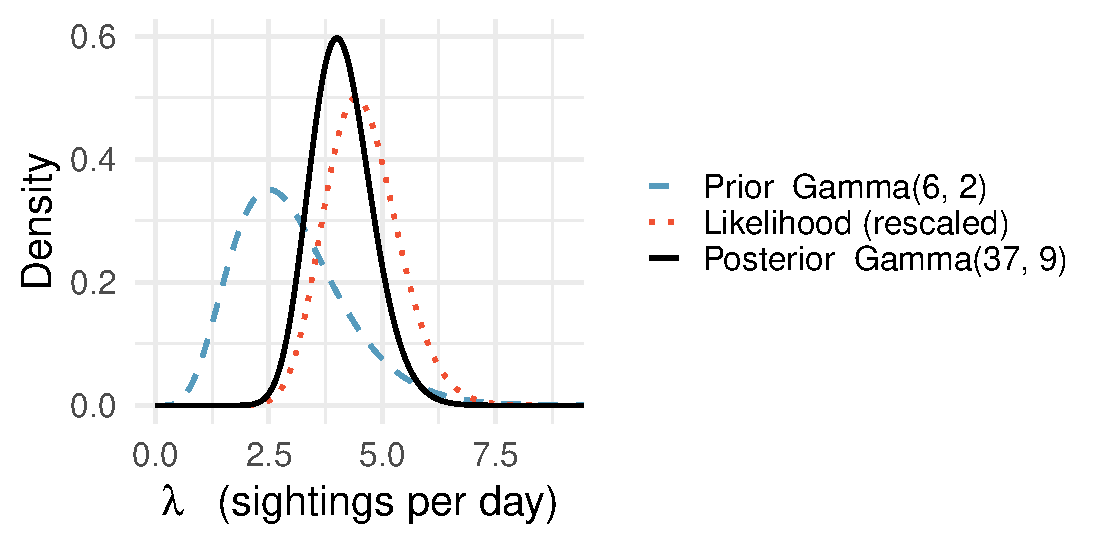
\includegraphics[width=0.86\textwidth]{gamma_poisson_update.pdf}
\end{center}

\vspace{-0.3em}
Three families, three pictures, one story: the posterior sits between the prior and the likelihood, and is narrower than either.

\end{frame}

%%%%%%%%%%%%%%%%%%%%%%%%%%%%%%%%%%%%%%%%%%%%%%%%%%%%%%%%%%%%%%%%%%%%%%%%
\section{Wrap-up}

%%%%%%%%%%%%%%%%%%%%%%%%%%%%%%%%%%%%%%%%%%%%%%%%%%%%%%%%%%%%%%%%%%%%%%%%
\begin{frame}
\frametitle{The three conjugate families}

\vspace{-0.2em}
\begin{center}
{\scriptsize
\renewcommand{\arraystretch}{1.5}
\begin{tabular}{lccc}
\toprule
 & \textbf{Beta-Binomial} & \textbf{Normal-Normal} & \textbf{Gamma-Poisson} \\
\midrule
Parameter & probability $p$ & mean $\mu$ & rate $\lambda$ \\
Data & $\text{Bin}(n,p)$ & $N(\mu, \sigma^2)$ & $\text{Pois}(\lambda)$ \\
Prior & $\text{Beta}(\alpha,\beta)$ & $N(\mu_0, \sigma_0^2)$ & $\text{Gamma}(\alpha,\beta)$ \\
Posterior & $\text{Beta}(\alpha\!+\!x,\; \beta\!+\!n\!-\!x)$ & $N(\mu_n, \sigma_n^2)$ & $\text{Gamma}(\alpha\!+\!\textstyle\sum x_i,\; \beta\!+\!n)$ \\
\textbf{Prior size $n_0$} & $\alpha + \beta$ & $\sigma^2/\sigma_0^2$ & $\beta$ \\
\bottomrule
\end{tabular}}
\end{center}

\pause
{\small Only the bottom row differs. Once you know $n_0$, the posterior mean is the same weighted average every time.}

\end{frame}

%%%%%%%%%%%%%%%%%%%%%%%%%%%%%%%%%%%%%%%%%%%%%%%%%%%%%%%%%%%%%%%%%%%%%%%%
\begin{frame}
\frametitle{Limitations of conjugate priors}

\hl{What they buy you:}
\begin{itemize}
\item a posterior in closed form: no computation, just arithmetic on the parameters;
\item parameters you can read aloud: ``prior successes,'' ``prior sample size'';
\item sequential updating for free.
\end{itemize}

\pause
\medskip

\hl{What they cost you:}
\begin{itemize}
\item the conjugate prior may \emph{not} be what you believe: what if your prior should be bimodal, or heavy-tailed?
\pause
\item conjugacy holds only for a few prior/likelihood pairs. Most real models have \textbf{no conjugate prior at all}.
\end{itemize}

\end{frame}

%%%%%%%%%%%%%%%%%%%%%%%%%%%%%%%%%%%%%%%%%%%%%%%%%%%%%%%%%%%%%%%%%%%%%%%%
\begin{frame}
\frametitle{Summary}

\begin{itemize}
\item A prior is \hl{conjugate} to a likelihood when the posterior comes out in the same family: Beta/Binomial, Normal/Normal, Gamma/Poisson.
\pause
\item The update is then pure bookkeeping: \hl{add the data to the prior's parameters}. No integration.
\pause
\item In all three, the \hl{posterior mean is a weighted average} of the prior mean and the MLE, with weights $\frac{n_0}{n_0+n}$ and $\frac{n}{n_0+n}$.
\pause
\item The \hl{prior sample size $n_0$} says how many observations your prior is worth. It is the only thing that changes between families.
\pause
\item With enough data the prior washes out and the posterior mean approaches the MLE.
\end{itemize}

\end{frame}

%%%%%%%%%%%%%%%%%%%%%%%%%%%%%%%%%%%%%%%%%%%%%%%%%%%%%%%%%%%%%%%%%%%%%%%%
\begin{frame}
\frametitle{Coming up next}

\hl{Conjugacy was the easy case}, and a rare one. Closed-form posteriors come only from the handful of prior/likelihood pairs that multiply into their own family.

\vspace{0.4em}
\begin{itemize}
\item \hl{Lecture 19: posterior approximation.} With no conjugate prior, which is most of the time, you cannot write the posterior down. So you \emph{sample} from it instead, with \hl{Markov chain Monte Carlo}, and study the draws (BR!\ Chs.\ 6--7).
\pause
\item That brings its own problem: the samples are only trustworthy if the chain behaved. Hence \hl{trace plots} and the diagnostics \hl{R-hat} and \hl{ESS}, which decide whether the output is usable.
\end{itemize}

\end{frame}

%%%%%%%%%%%%%%%%%%%%%%%%%%%%%%%%%%%%%%%%%%%%%%%%%%%%%%%%%%%%%%%%%%%%%%%%
\begin{frame}
\frametitle{In-class activity}

You'll work in \textbf{pairs} (one analyst, one guide).

\medskip
\begin{itemize}
\item Pick up the worksheet.
\item Work through the problems together.
\item \hl{Don't use Gen AI except for debugging}
\item Your worksheet will be collected and graded.
\end{itemize}

\medskip
\textbf{Recommendations:}
\begin{itemize}
\item Read each question carefully before starting
\item Discuss your answers with your partner before writing them down.
\end{itemize}

\end{frame}

\end{document}
